\documentclass[final,hyperref={pdfpagelabels=false}]{beamer}
\mode<presentation>{\usetheme{I6pd2}}
\usepackage[orientation=landscape,size=a0,scale=1.4,debug]{beamerposter}
\usepackage[english]{babel}
\usepackage[latin1]{inputenc}
\usepackage{color}
\usepackage{colortbl}
\usepackage{array,booktabs,tabularx}
\usepackage{tikz}
\usetikzlibrary{shapes.arrows}

\definecolor{OrangeRed}{RGB}{255, 40, 0}
\tikzset{
    myarrow/.style={
        draw,
        fill=OrangeRed,
        single arrow,
        minimum height=4.5ex,
        single arrow head extend=1.5ex
    }
}
\newcommand{\arrowdig}{%
\tikz [baseline=-0.5ex]{\node [myarrow,rotate=45] {};}
}
%%%%%%%%%%%%%%%%%%%%%%%%%%%%%%%%%%%%%%%%%%%%%%%%%%%%%%%%%%%%%%%%%%%%%%%%%%%%%%%%%%%%%%

%\usepackage{mathastext}
%\everymath{\scriptstyle}
%\usepackage{grffile}
%\usepackage{amsmath,amsthm, amssymb, latexsym}
%\usepackage{setspace}
%\usepackage{ragged2e}
%\usepackage{relsize}
%\newcolumntype{Z}{>{\centering\arraybackslash}X} % centered tabularx columns
%\newcommand{\pphantom}{\textcolor{ta3skyblue}} % phantom introduces a vertical space in p formatted table columns??!!
%\listfiles

%%%%%%%%%%%%%%%%%%%%%%%%%%%%%%%%%%%%%%%%%%%%%%%%%%%%%%%%%%%%%%%%%%%%%%%%%%%%%%%%%%%%%%

\title{\Large COMBINING CRITERIA FOR THE DETECTION OF INCORRECT ENTRIES OF NON-NATIVE SPEECH\\\vskip1ex IN THE CONTEXT OF FOREIGN LANGUAGE LEARNING}

\author{Luiza Orosanu, Denis Jouvet, Dominique Fohr, Irina Illina , Anne Bonneau\\
Speech Group, LORIA (Inria, CNRS, Universite de Lorraine)\\
Nancy, France}
\date[December. 5th, 2012]{December. 5th, 2012}

%%%%%%%%%%%%%%%%%%%%%%%%%%%%%%%%%%%%%%%%%%%%%%%%%%%%%%%%%%%%%%%%%%%%%%%%%%%%%%%%%%%%%%
\newlength{\columnheight}
\setlength{\columnheight}{105cm}

%%%%%%%%%%%%%%%%%%%%%%%%%%%%%%%%%%%%%%%%%%%%%%%%%%%%%%%%%%%%%%%%%%%%%%%%%%%%%%%%%%%%%%
\begin{document}
\begin{frame}
\begin{columns}
% ---------------------------------------------------------%
% Set up a column
\begin{column}{.40\textwidth}
\begin{beamercolorbox}[center,wd=\textwidth]{postercolumn}
\begin{minipage}[T]{.95\textwidth}
\parbox[t][\columnheight]{\textwidth}{

\begin{block}{Introduction}
      \begin{itemize}
      \item How does an \textcolor{OrangeRed}{automatic system for foreign language learning} work?
	\begin{itemize}
		\item the system displays a word or a sentence on the screen
		\item the learner must pronounce and record the expected sentence
		\item the system analyzes the acoustic signal that has just been recorded
		\item the learner receives the feed-back on the quality of his pronunciation
	\end{itemize}
      \item What could go wrong?
        \begin{itemize}
        \item the learner could be distracted by the environment
        \item the learner might pronounce a different sentence, or skip a few words
       	\item a technical problem might appear during the recording
	\end{itemize}
      \item \textcolor{OrangeRed}{\textbf{What is our objective?}}
        \begin{itemize}
        \item introduce a detector of incorrect entries before starting the analysis
        \item make sure that the received data can be considered as being "correct"
        \end{itemize}
      \end{itemize}
    \end{block}

    \vskip1ex
    \begin{block}{Decode the audio signals in three different ways}
      	\begin{itemize}
       		\item \textcolor{OrangeRed}{Constrained decoding}: the system is forced to follow the sequence of words within the expected text
     		\item \textcolor{OrangeRed}{Phonetic decoding based on phoneme loop}: the system is free to choose any phoneme in any position in the sentence
       		\item \textcolor{OrangeRed}{Phonetic decoding based on word loop}: the system is free to choose any word in any position in the sentence
	\end{itemize}
    \end{block}

    \vskip1ex
    \begin{block}{Compare a constrained decoding with an unconstrained one}
	\noindent

	\begin{itemize}
		\item Comparison criteria associated to the \textcolor{OrangeRed}{phonemes}: measures the phonemes adequacy
			\begin{columns}
				\begin{column}{0.50\textwidth} \hfill\includegraphics[scale=1.1]{Image/criteria/ph_correct.png}\end{column}
				\begin{column}{0.50\textwidth} \begin{center}\includegraphics[scale=1]{Image/criteria/ph_incorrect.png}\end{center}\end{column}
			\end{columns}
			\textcolor{ta3skyblue}{\rule[0.1ex]{0.97\textwidth}{1.6pt}}
%
		\item Comparison criteria associated to the \textcolor{OrangeRed}{frames}: measures the phonetic class adequacy
			\begin{columns}
				\begin{column}{0.50\textwidth} \hfill\includegraphics[scale=1]{Image/criteria/tr_correct.png}\end{column}
				\begin{column}{0.50\textwidth} \begin{center}\includegraphics[scale=1]{Image/criteria/tr_incorrect.png}\end{center}\end{column}
			\end{columns}
			\textcolor{ta3skyblue}{\rule[0.1ex]{0.97\textwidth}{1.6pt}}
%
		\item Comparison criteria associated to the \textcolor{OrangeRed}{non-speech segments}: measures the duration difference of non-speech segments
			\begin{columns}
				\begin{column}{0.50\textwidth} \begin{center}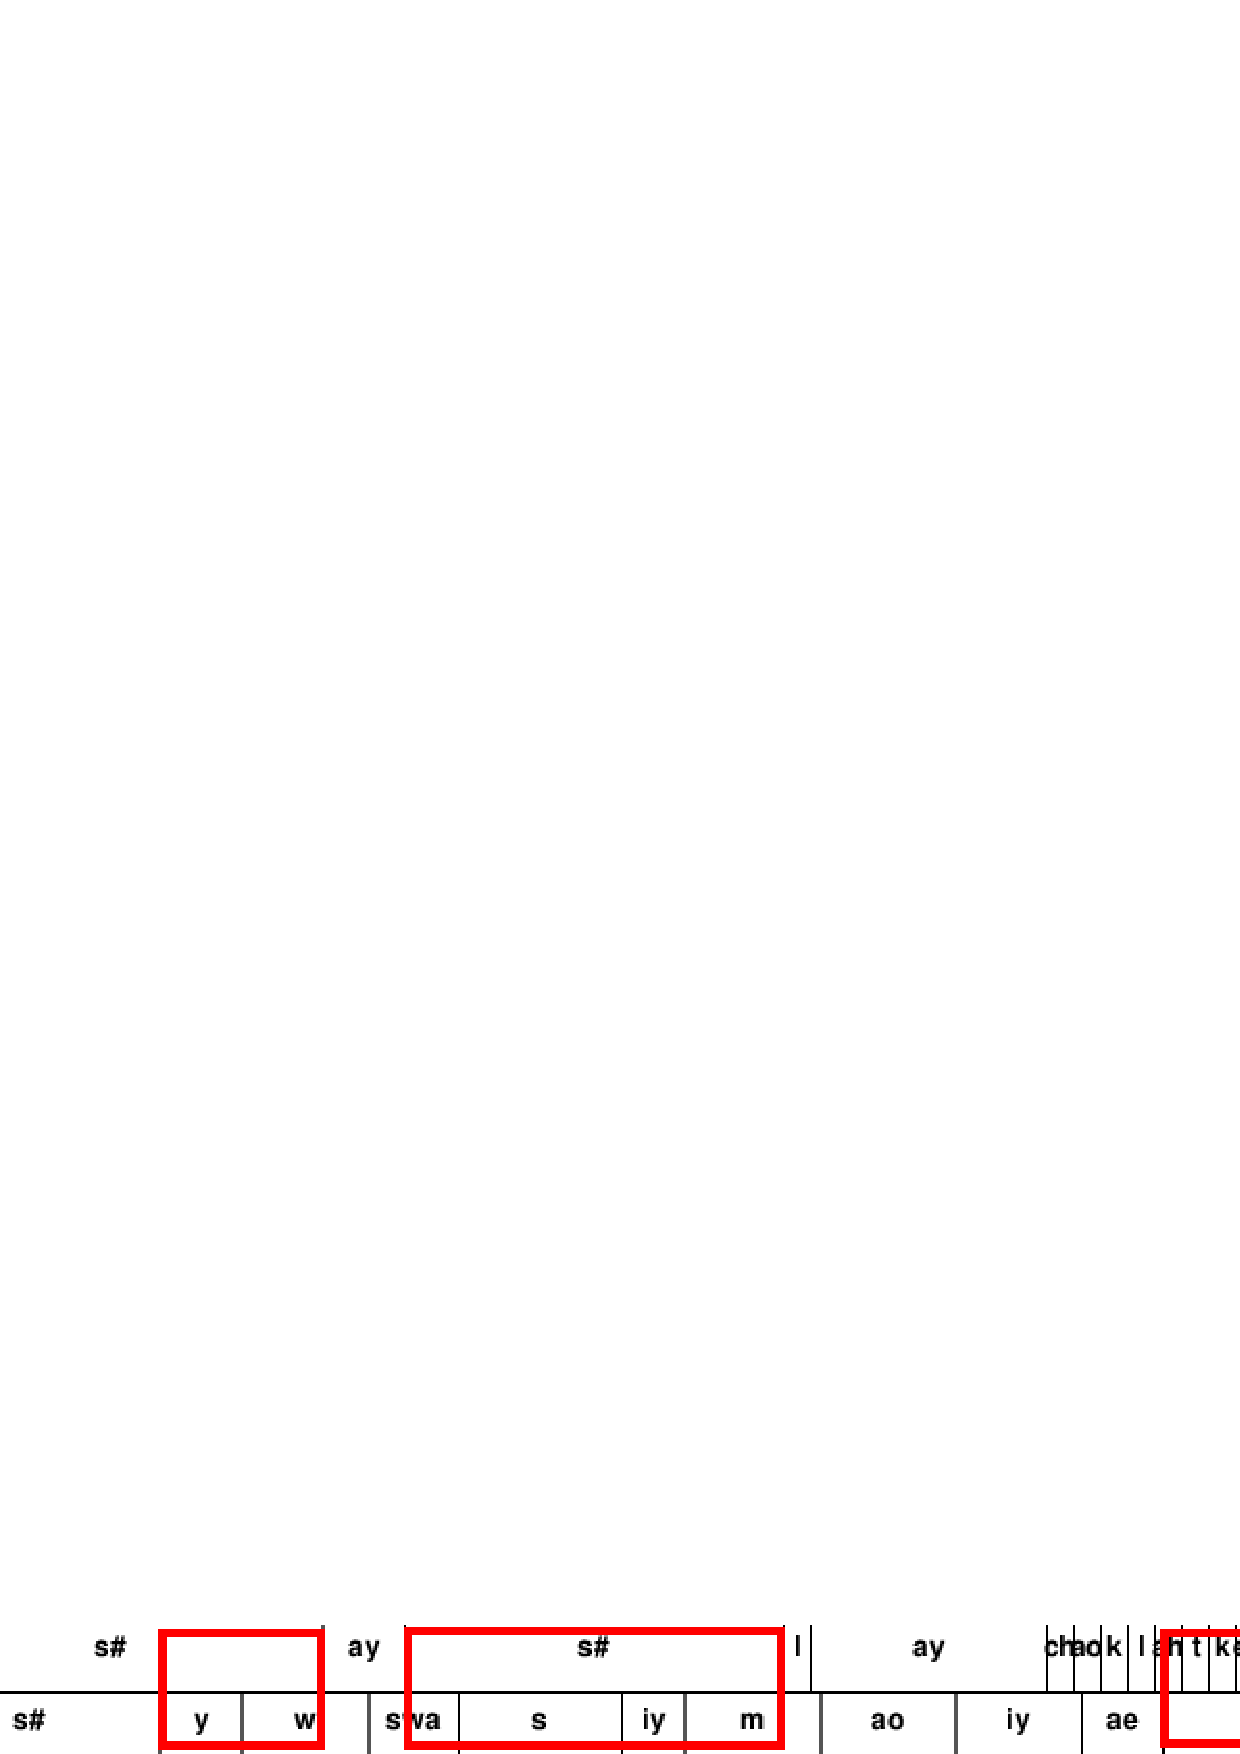
\includegraphics[scale=1]{Image/criteria/sil.png}\end{center}\end{column}
			\end{columns}
			\textcolor{ta3skyblue}{\rule[0.1ex]{0.97\textwidth}{1.6pt}}
%
		\item Comparison criteria associated to the \textcolor{OrangeRed}{log likelihood ratio}: measures the difference between the logarithmic likelihoods
			\textcolor{ta3skyblue}{\rule[0.1ex]{0.97\textwidth}{1.6pt}}
%
		\item Comparison criteria associated to the \textcolor{OrangeRed}{phonemes of minimal duration}: measures the difference between the number of short phonemes
			\begin{columns}
				\begin{column}{0.50\textwidth} \hfill\includegraphics[scale=1]{Image/criteria/dur_correct.png}\end{column}
				\begin{column}{0.50\textwidth} \begin{center} \includegraphics[scale=1]{Image/criteria/dur_incorrect.png}\end{center}\end{column}
			\end{columns}
	\end{itemize}
    \end{block}
  }
\end{minipage}
\end{beamercolorbox}
\end{column}
% ---------------------------------------------------------%
% end the column


    % ---------------------------------------------------------%
    % Set up a column
    \begin{column}{.33\textwidth}
      \begin{beamercolorbox}[center,wd=\textwidth]{postercolumn}
        \begin{minipage}[T]{.95\textwidth}
          \parbox[t][\columnheight]{\textwidth}{

            \begin{block}{Entry classifier}
              \begin{itemize}
		\item Define the \textcolor{OrangeRed}{training data set} $\mathrm{D=\{\bar{X}_{i}, y_{i}\}, i=1,...,N}$ where:
			\begin{center}
			\begin{itemize}
			\item $\mathrm{\bar{X}_{i} = \{x_1, x_2,..., x_k\}}$ is the vector containing \textcolor{OrangeRed}{\textbf{\textit{k}}} comparison criteria
			\item $\mathrm{y_i}$ = 1 (correct entry) or 0 (incorrect entry)
			\item $\mathrm{N}$ = the number of entries within the training data set
			\end{itemize}
			\end{center}
		\textcolor{ta3skyblue}{\rule[0.1ex]{0.95\textwidth}{1.6pt}}

               	\item Compute an entry's probability of being correct (\textcolor{OrangeRed}{logistic regression})\\
               		\begin{center} $\mathrm{f(\bar{X})=\frac{1}{1+exp(-(\alpha _{0}+\alpha _{1}x_{1}+\alpha _{2}x_{2}+...+\alpha _{k}x_{k}))}}$ \end{center}
		\textcolor{ta3skyblue}{\rule[0.1ex]{0.95\textwidth}{1.6pt}}

               	\item Estimate the \textcolor{OrangeRed}{$\mathrm{\alpha}$} parameters by minimizing the \textcolor{OrangeRed}{error function}
			\begin{center} $\mathrm{E=-\sum_{i=1}^{N}\left ( y_i\cdot ln(f(\bar{X}_i))+(1-y_i)\cdot ln(1-f(\bar{X}_i \right )}$ \end{center}
		\textcolor{ta3skyblue}{\rule[0.1ex]{0.95\textwidth}{1.6pt}}

               	\item Evaluate the classifier's performance
			\begin{itemize}
				\item compute error rates for various values of a \textcolor{OrangeRed}{$\mathrm{0\leq\sigma\leq1}$} threshold\vskip1ex
				\item if \textcolor{OrangeRed}{$\mathrm{f(\bar{X}) > \sigma}$} then the entry represented by the $\mathrm{\bar{X}}$ criteria  is accepted\vskip1ex
				\item \textcolor{OrangeRed}{False Acceptance} $\mathrm{FA=\frac{incorrect\;entries\;wrongly\;rejected}{incorrect\;entries}}$\vskip1ex
				\item \textcolor{OrangeRed}{False Rejection}  $\mathrm{FR=\frac{correct\;entries\;wrongly\;rejected}{correct\;entries}}$\vskip1ex
				\item \textcolor{OrangeRed}{F-measure}        $\mathrm{\frac{1}{F}=\frac{1}{2}\left ( \frac{1}{1-FA}+\frac{1}{1-FR} \right )}$
			\end{itemize}
              \end{itemize}
            \end{block}

	  \vskip0.2ex
          \begin{block}{Experimental setup}
              \begin{itemize}
               	\item \textcolor{OrangeRed}{Non-native corpora}
	              \begin{itemize}
			\item INTONALE Project
			\item $\sim$ 800 English sentences
			\item 34 French speakers (29 women, 5 men) \hfill\arrowdig
			\item 50\% for training, 50\% for testing (results displayed on poster)
             	      \end{itemize}
		\textcolor{ta3skyblue}{\rule[0.1ex]{0.95\textwidth}{1.6pt}}

               	\item \textcolor{OrangeRed}{Native corpora}
	              \begin{itemize}
			\item INTONALE Project
			\item $\sim$ 1500 English sentences
			\item 22 English speakers (15 women, 7 men)
			\item 50\% for training, 50\% for testing (results presented in the paper)
             	      \end{itemize}
		\textcolor{ta3skyblue}{\rule[0.1ex]{0.95\textwidth}{1.6pt}}

               	\item HMM toolkit: \textcolor{OrangeRed}{HTK}\vskip1ex
               	\item Acoustic features: \textcolor{OrangeRed}{MFCC} (12 MFCC coefficients + temporal derivates + the logarithm of the energy per frame)\vskip1ex
               	\item Acoustic models: \textcolor{OrangeRed}{HMM} (16 gaussian mixtures)\vskip1ex
               	\item Two lexicons:
			\begin{itemize}
				\item native (CMU)
				\item non-native (includes non-native variants)
			\end{itemize}
              \end{itemize}
            \end{block}
	   }
        \end{minipage}
      \end{beamercolorbox}
    \end{column}
    % ---------------------------------------------------------%
    % end the column


    % ---------------------------------------------------------%
    % Set up a column
    \begin{column}{.27\textwidth}
      \begin{beamercolorbox}[center,wd=\textwidth]{postercolumn}
        \begin{minipage}[T]{.95\textwidth}
          \parbox[t][\columnheight]{\textwidth}{

            \begin{block}{Impact of the lexicon and the training data set}
		\begin{columns}
			\begin{column}{.55\textwidth}
				\begin{center}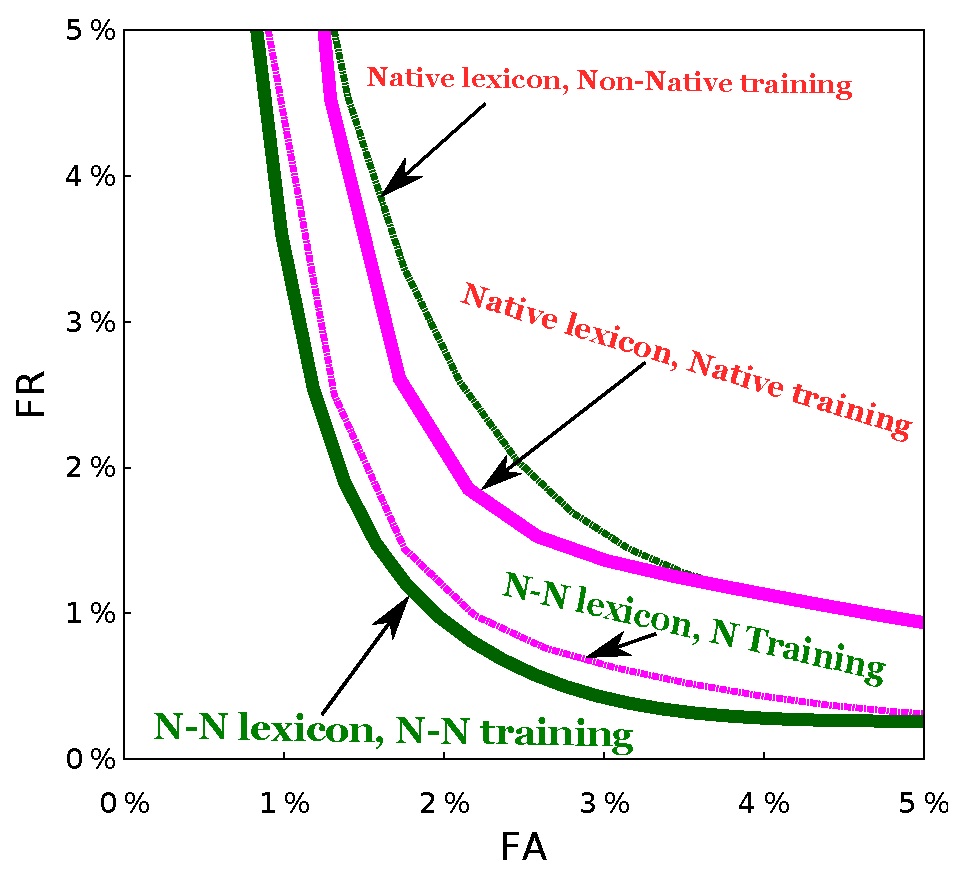
\includegraphics{Image/curves/courbeDET_MAC_lex_training}\end{center}
			\end{column}
			\begin{column}{.44\textwidth}
				\begin{itemize}
					\item non-native lexicon
					\item non-native training data set
				\end{itemize}
			\end{column}
		\end{columns}
	   \end{block}

	    \vskip0.7ex
            \begin{block}{Impact of the comparison criteria}
		\begin{columns}
			\begin{column}{.55\textwidth}
				\begin{center}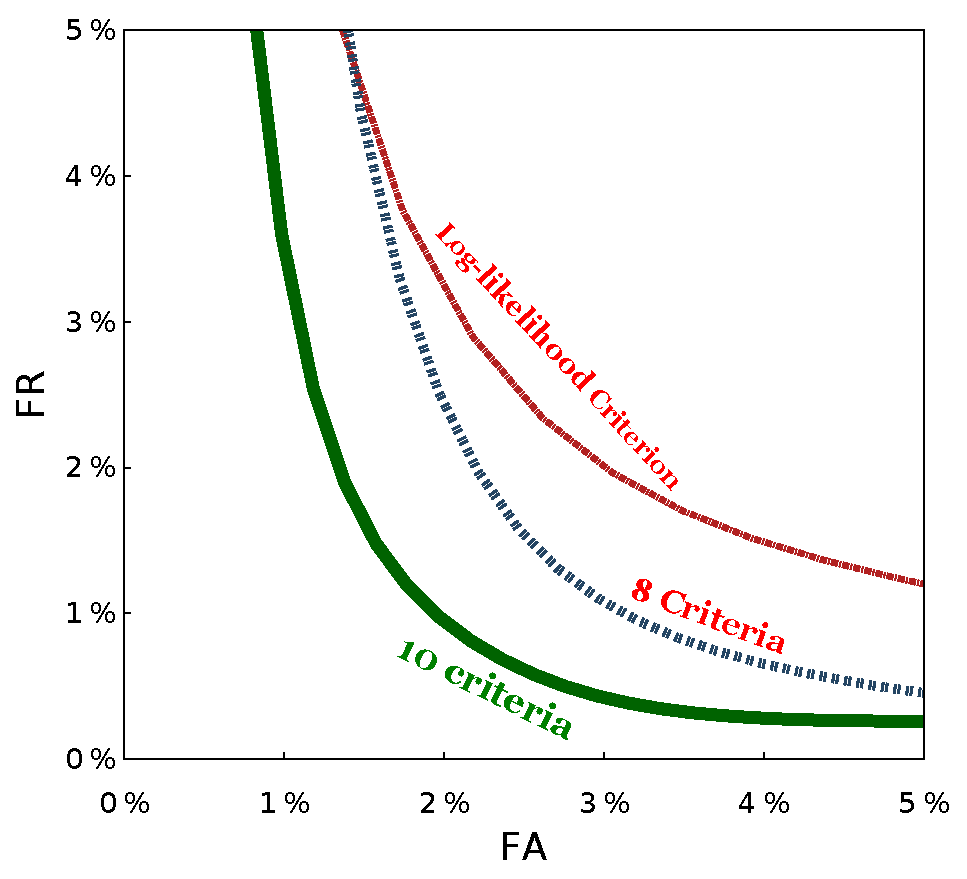
\includegraphics{Image/curves/courbeDET_MAC_criteria}\end{center}
			\end{column}
			\begin{column}{.44\textwidth}
				\begin{itemize}
					\item comparison of the forced alignment with both phoneme loop and word loop alignments
					\item all 10 comparison criteria (5 criteria per comparison)
				\end{itemize}
			\end{column}
		\end{columns}
            \end{block}

	    \vskip0.7ex
	    \begin{block}{Overall performance}
		\begin{columns}
			\begin{column}{.49\textwidth}
				\begin{center}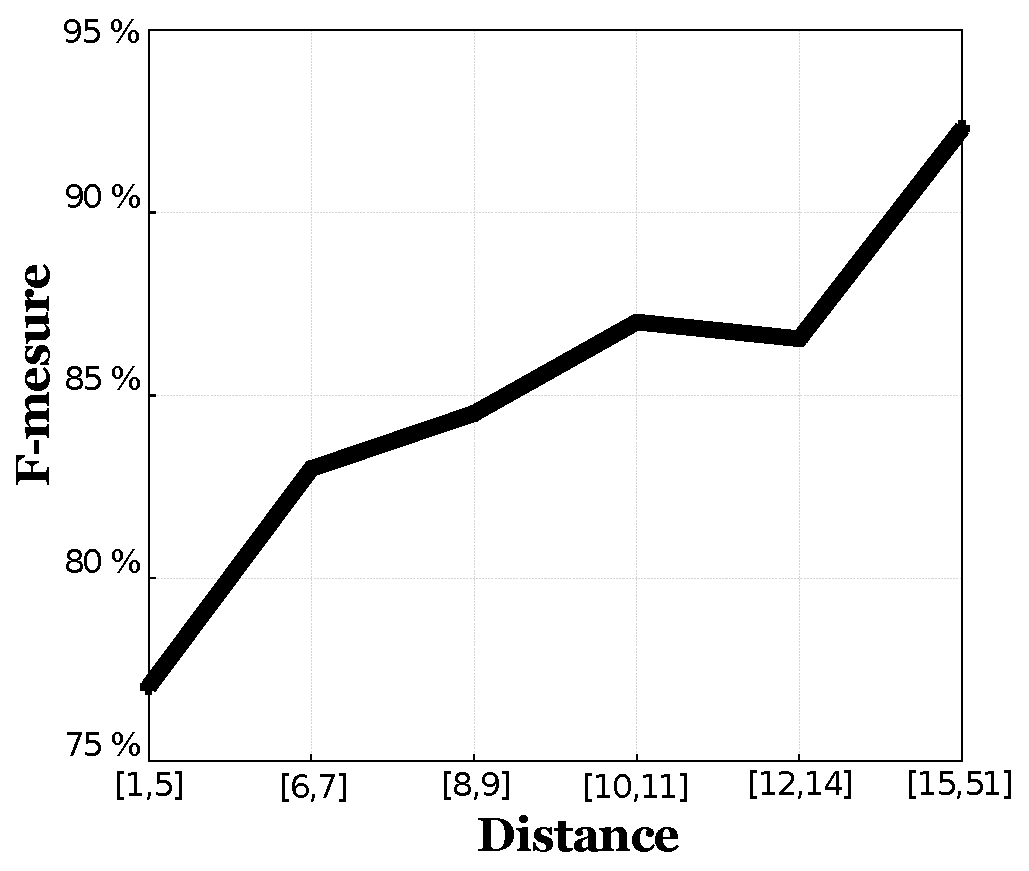
\includegraphics[scale=0.85]{Image/curves/allStats_curve_NN} \end{center}
			\end{column}
			\begin{column}{.50\textwidth}
				\begin{itemize}
					\item distance: measures the difference between the original correct transcription (which should be accepted) and the modified transcription (which should be rejected)
				\end{itemize}
			\end{column}
		\end{columns}
		\begin{itemize}\item the F-measure gets greater than 80\% when difference over 6 phonemes\end{itemize}
            \end{block}

	    \vskip0.8ex
            \begin{block}{Conclussions}
		\begin{itemize}
		\item Our experiments have shown that it is important to:
		      \begin{itemize}
		       	\item train the decision function on non-native data
		       	\item use non-native pronunciations in the lexicon
		       	\item combine all 10 comparison criteria
		      \end{itemize}
		\item The optimal setting leads to a classifier able to detect incorrect entries when more than 6 phonemes are wrong
		\end{itemize}
            \end{block}


          }
        \end{minipage}
      \end{beamercolorbox}
    \end{column}
    % ---------------------------------------------------------%
    % end the column
  \end{columns}
  \vskip1ex
\end{frame}
\end{document}


%%%%%%%%%%%%%%%%%%%%%%%%%%%%%%%%%%%%%%%%%%%%%%%%%%%%%%%%%%%%%%%%%%%%%%%%%%%%%%%%%%%%%%%%%%%%%%%%%%%%
%%% Local Variables:
%%% mode: latex
%%% TeX-PDF-mode: t
%%% End:
